\documentclass[../relatorio.tex]{subfiles}
\begin{document}
A partir da análise dos requisitos funcionais, em particular dos casos de uso,
decidiu-se construir um Diagrama de Componentes (\ref{img:diagrama_componentes}) que visa, neste caso,
estruturar o projeto por camadas, correspondendo estas a sistemas:
\begin{itemize}
    \item[ReparacoesUI]{
          Camada de interação com o utilizador.
          }
    \item[ReparacoesLN]{
          Camada de lógica do negócio, engloba todo o conhecimento sobre estado
          da aplicação, assim como o manusear.
          }
    \item[ReparacoesBD] {
          Camada de acesso a base de dados. \\
          \textit{Neste projeto, esta camada foi simplificada devido
              à falta de conhecimento dos elementos}
          }
\end{itemize}

\subsubsection*{ReparacoesUI} \label{sec:reparacoes_ui}
Como já referido, refere-se à camada de interação com o utilizador.
Utiliza API da \textbf{ReparacoesLN} (ver \ref{sec:reparacoes_ln}).

Desta forma, o modo de interação com o utilizador pode ser modificado na sua totalidade
sem que haja necessidade de qualquer alteração ao nível da camada de lógica.

\subsubsection*{ReparacoesLN} \label{sec:reparacoes_ln}
O sistema da lógica do negócio, expõe uma interface designada \textit{IReparacoesLN}, por forma a garantir o encapsulamento do mesmo.
Esta estratégia permite que o sistema que o utiliza (neste caso, \textbf{ReparacoesUI})
não dependa da sua implementação, isolando a implementação lógica.
Não obstante, esta divisão inicial, foi identificado um conjunto de subsistemas que permitiram
uma melhor organização, implementação e manutenção do projeto, procurando diminuir as suas dependências.
Assim, identificou-se três subsistemas: \underline{SSClientes}, \underline{SSReparacoes}, \underline{SSColaboradores}.
Utiliza a camada de base de dados (ver \ref{sec:reparacoes_bd}) por forma a garantir a persistência do estado da
aplicação entre utilizações.

\begin{itemize}
    \item[\textbf{SSClientes}] {
          Realiza a interface \textit{IGestClientes}.\\
          Engloba a lógica relacionada com os Clientes (\ref{ent_cliente})
          e os seus Equipamentos (\ref{ent_equipamento}).
          }
    \item[\textbf{SSColaboradores}] {
          Realiza a interface \textit{IGestColaboradores}.\\
          Engloba toda a lógica relacionada com os Colaboradores (\ref{ent_colaborador})
          e as suas especializações e o balcão.
          Tem, ainda, a Gestão da Agenda dos Colaboradores.
          Esta funcionalidade derivou da necessidade dos técnicos terem uma lista de reparações
          e passar a ser possível fazer uma estimativa do prazo de reparação, sempre que é adicionada
          uma nova.
          }
    \item[\textbf{SSReparacoes}] {
          Realiza a interface \textit{IGestReparacoes}.\\
          Engloba toda a lógica relacionada com as Reparações (\ref{ent_reparacao})
          e com os Orcamentos (\ref{ent_orcamento}).
          }
\end{itemize}

\subsubsection*{ReparacoesBD} \label{sec:reparacoes_bd}
Conforme referido, a camada de base de dados deste projeto corresponde,
na realidade, a uma simples persistência do estado de toda a aplicação
armazenado num ficheiro de objetos.

No entanto, optou-se por colocar uma camada específica para este efeito
por forma a manter a garantia de facilidade de manutenção e uma eventual
implementação de um sistema de base de dados.

Para tal, realiza a interface \textbf{IReparacoesBD}.

\begin{figure}[!ht]
    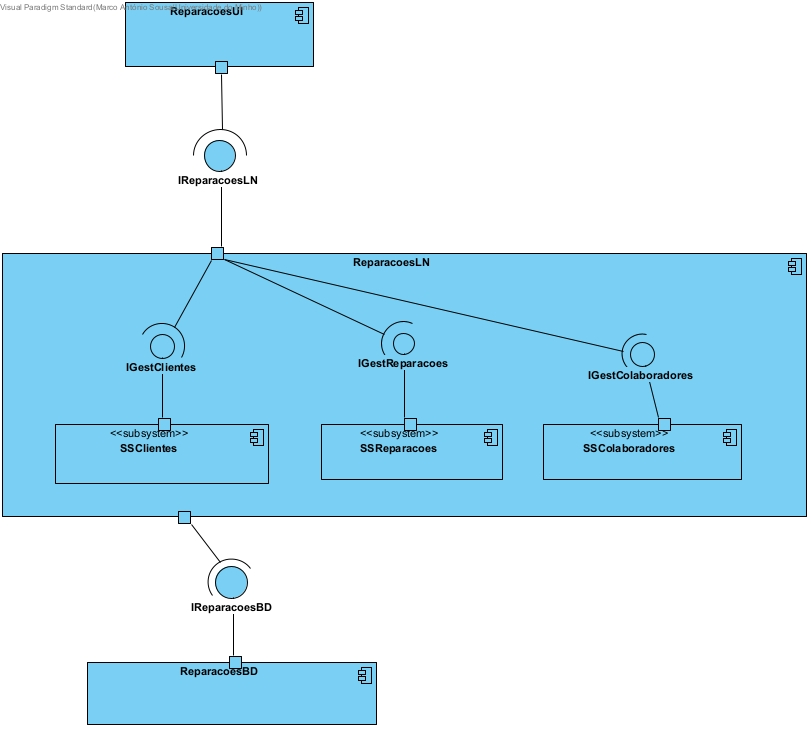
\includegraphics[width=\textwidth]{componente.jpg}
    \caption{Diagrama de Componentes} \label{img:diagrama_componentes}
\end{figure}

\end{document}